%% LyX 2.2.3 created this file.  For more info, see http://www.lyx.org/.
%% Do not edit unless you really know what you are doing.
\documentclass[english]{article}
\usepackage[T1]{fontenc}
\usepackage[utf8]{inputenc}
\usepackage{geometry}
\geometry{verbose,rmargin=3cm,bmargin=2cm, footskip=1cm, tmargin=2cm}
\usepackage{float}
\usepackage{textcomp}
\usepackage{graphicx}
\usepackage{hyperref}
\hypersetup{colorlinks=true}
\usepackage{color}
\definecolor{mygray}{rgb}{1,0.98,0.98}
\definecolor{myred}{rgb}{1,0.60,1}
\makeatletter

%%%%%%%%%%%%%%%%%%%%%%%%%%%%%% LyX specific LaTeX commands.
%% Because html converters don't know tabularnewline
\providecommand{\tabularnewline}{\\}

\@ifundefined{date}{}{\date{}}
%%%%%%%%%%%%%%%%%%%%%%%%%%%%%% User specified LaTeX commands.

\usepackage{array}
\usepackage{color}
\usepackage{colortbl}

\makeatother

\usepackage{babel}
\usepackage{listings}
\renewcommand{\lstlistingname}{Listing}

\title{Tutorato Architettura degli Elaboratori Modulo 2 \\ Lezione 1}
\author{Francesco Pelosin}
\date{9 Marzo 2020}

\begin{document}
\lstset{frame=single, numbers=left, backgroundcolor=\color{mygray}}
\maketitle

\section{Instruction Level Parallelism}

La semplice pipeline usata per eseguire il set di istruzioni ristretto (\texttt{lw,sw,add,or,beq,slt}) del nostro processore MIPS è composta da 5 stadi:

\begin{enumerate}
    \item \texttt{IF} : Instruction fetch (memoria istruzioni)
    \item \texttt{ID} : Instruction decode e lettura registri
    \item \texttt{EXE} : Esecuzione istruzioni e calcolo indirizzi
    \item \texttt{MEM} : Accesso alla memoria (memoria dati)
    \item \texttt{WB} : Write back (scrittura del registro risultato, calcolato in \texttt{EXE} o \texttt{MEM})

\end{enumerate}
\begin{figure}[H]
    \centering
    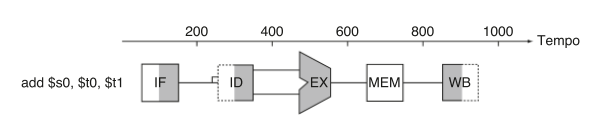
\includegraphics[width=1\textwidth]{im00.png}
    \caption{Rappresentazione grafica di una istruzione nella pipeline.}
    \label{fig:im00}
\end{figure}

\subsection*{Esercizio 1}

Considerare un processore con pipeline a 5 stadi senza forwarding, con un register
file non otimizzato\footnote{prima legge il vecchio valore di un registro e poi
lo scrive al ciclo di clock successivo}. Il processore è fornito di hazard detection unit, è quindi in grado
di mettere in stallo la pipeline.

\begin{lstlisting}
sub $3, $2, $5
lw $10, 4($3)
addi $3, $3, 8
add $20, $20, $10
\end{lstlisting}
Domande:
\begin{enumerate}
\item Determinare le dipendenze RAW tra le istruzioni del programma assembler
precedente.
\item Disegnare il diagramma temporale di esecuzione. 
\item Cosa succede all\textquoteright 8\textdegree{} ciclo di clock nei
vari stadi?
\item Se il processore non fosse dotato di hazard detection unit, dove dovrebbero
essere inserite le \texttt{nop} per evitare inconsistenze dovute alle dipendenze
sui dati? 
\end{enumerate}

\subsubsection*{Soluzione domanda 1} 
Dipendenze:
\begin{itemize}
    \item $1\rightarrow2$. L'istruzione 2 legge il registro \$3 precedentemente
scritto dall'istruzione 1.
    \item $2\rightarrow4$. L'istruzione 4 legge il registro \$10 precedentemente
scritto dall'istruzione 2.

\item Ci sarebbe anche la dipendenza $(1\rightarrow3)$, 
ma in realtà, visto il tipo di processore, l'istruzione 3 entra in stallo a
causa della dipendenza $(1\rightarrow2)$ e quando ne esce ha il dato disponibile
senza ulteriori ritardi.
\end{itemize}

\subsubsection*{Soluzione domanda 2}


\begin{tabular}{|c|c|c|c|c|c|c|c|c|c|c|c|c|c|c|}
\cline{3-15} 
\multicolumn{1}{c}{} &  & {\tiny{}1} & {\tiny{}2} & {\tiny{}3} & {\tiny{}4} & {\tiny{}5} & {\tiny{}6} & {\tiny{}7} & {\tiny{}8} & {\tiny{}9} & {\tiny{}10} & {\tiny{}11} & {\tiny{}12} & {\tiny{}13}\tabularnewline
\hline 
{\scriptsize{}1} & {\scriptsize{}sub} & {\tiny{}IF} & {\tiny{}ID} & {\tiny{}EXE} & {\tiny{}MEM} & {\tiny{}WB} &  &  &  &  &  &  &  & \tabularnewline
\hline 
{\scriptsize{}2} & {\scriptsize{}lw} &  & {\tiny{}IF} & {\tiny{}ID} & {\tiny{}\cellcolor[\color{myred}]{.9}<ID>} & {\tiny{}\cellcolor[\color{myred}]{.9}<ID>} & {\tiny{}\cellcolor[\color{myred}]{.9}<ID>} & {\tiny{}EXE} & {\tiny{}MEM} & {\tiny{}WB} &  &  &  & \tabularnewline
\hline 
{\scriptsize{}3} & {\scriptsize{}addi} &  &  & {\tiny{}IF} & {\tiny{}\cellcolor[\color{myred}]{.9}<IF>} & {\tiny{}\cellcolor[\color{myred}]{.9}<IF>} & {\tiny{}\cellcolor[\color{myred}]{.9}<IF>} & {\tiny{}ID} & {\tiny{}EXE} & {\tiny{}MEM} & {\tiny{}WB} &  &  & \tabularnewline
\hline 
{\scriptsize{}4} & {\scriptsize{}add} &  &  &  &  &  &  & {\tiny{}IF} & {\tiny{}ID} & {\tiny{}\cellcolor[\color{myred}]{.9}<ID>} & {\tiny{}\cellcolor[\color{myred}]{.9}<ID>} & {\tiny{}EXE} & {\tiny{}MEM} & {\tiny{}WB}\tabularnewline
\hline 
\end{tabular}
\subsubsection*{Soluzione domanda 3}

All'ottavo ciclo i vari stadi eseguono quanto segue:
\begin{itemize}
\item \texttt{IF}: opera sull'eventuale quinta istruzione, di cui non sappiamo niente
perchè non data.
\item \texttt{ID}: esegue la decodifica della quarta istruzione (\texttt{add}).
\item \texttt{EXE}: esegue la terza istruzione (\texttt{addi}).
\item \texttt{MEM}: legge la memoria per la seconda istruzione (\texttt{lw}).
\item \texttt{WB}: è in attesa (bolla).
\end{itemize}

\subsubsection*{Soluzione domanda 4}
Se il processore non fosse dotato di hazard detection unit le \texttt{nop} andrebbero inserite come segue:
\begin{lstlisting}[numbers=none]
sub $3, $2, $5
nop
nop
nop
lw $10, 4($3)
addi $3, $3, 8
nop
nop
add $20, $20, $10
\end{lstlisting}
Notare che le \texttt{nop} inserite corrispondono alle bolle del diagramma temporale.

\newpage

\subsection*{Esercizio 2}
Si consideri il seguente programma.
\begin{lstlisting}
ori $6, $0, 0
ori $7, $0, 1000
loop:
    sll $5, $6, 2 #moltiplico per 4
    add $8, $4, $5
    lw $9, 0($8)
    and $9, $9, $0
    sw $9, 0($8)
    addi $6, $6, 1
    bne $6, $7, loop
\end{lstlisting}
Domande:
\begin{enumerate}
    \item Assumendo che \$4 contenga l’indirizzo di un vettore di interi, cosa fa questo codice?
    \item Determinare il $CPI$ del programma nel caso in cui il processore sia multiciclo (si ipotizzi che tutte le istruzioni R e I di tipo aritmentico/logico impieghino 4 cicli di clock, \texttt{lw} 5, \texttt{bne} 3).
    \item Rispetto all’implementazione multiciclo a pipeline vista a lezione (5 stadi, forwarding e delayed branch), dove si verificano eventuali stalli? Inserire le istruzioni \texttt{nop} opportune, e ricalcolare il $CPI$, senza considerare i cicli persi per il riempimento della pipeline.
\end{enumerate}

\subsubsection*{Soluzione domanda 1}
Il programma pone a 0 un vettore di interi di 1000 elementi.

\subsubsection*{Soluzione domanda 2}
Per il processore multicilco bisogna considerare che l'istruzione \texttt{bne} impiega 3 cicli, \texttt{lw} 5 cicli e tutte le altre istruzioni 4 cicli. Quindi abbiamo 8 cicli per il preambolo del loop, e $28 * 1000$ per il corpo del loop, per un totale di 28008 cicli. Il numero di istruzioni eseguite è $IC = 2 + 7 * 1000 = 7002$. Per cui abbiamo che:

$$CPI = \frac{28008}{7002} = 4$$


\subsubsection*{Soluzione domanda 3}
Per quanto riguarda il processore pipeline, abbiamo uno stallo dopo la \texttt{lw}, e dobbiamo forzare uno stallo dopo la \texttt{beq} a causa del delayed branch. Quindi il programma modificato è il seguente:

\begin{lstlisting}[numbers=none]
ori $6, $0, 0
ori $7, $0, 1000
loop:
    sll $5, $6, 2 #moltiplico per 4
    add $8, $4, $5
    lw $9, 0($8)
    nop
    and $9, $9, $0
    sw $9, 0($8)
    addi $6, $6, 1
    bne $6, $7, loop
    nop
\end{lstlisting}

Sono necessari quindi un numero di cicli pari a $2 + 9*1000 = 9002$. Per cui abbiamo che 

$$CPI = \frac{9002}{7002} = 1.286$$

\paragraph{N.B.} Se non contiamo il tempo per riempire la pipeline, il numero di cicli per istruzione è 1. Questo perché ad ogni di ciclo di clock una istruzione termina l'esecuzione, avendo così, 9002 cicli totali.

Contrariamente a quanto può sembrare il numero di istruzioni non è 9002 ma bensì 7002. Il $CPI$ è una statistica che calcoliamo prima che il compilatore inserisca le \texttt{nop}. Quindi, in parole povere, non le contiamo in quanto vengono inserite a posteriori dal compilatore e non rientrano nel calcolo della statistica.

\subsection*{Esercizio 3}

La tabella in Fig.~\ref{fig:im0} descrive la funzione usuale dei registri ed il
loro nome. Nei listati i registri possono venir chamati col numero
oppure col nome. 

\begin{figure}[H]
    \centering
    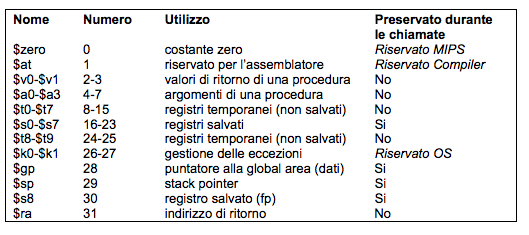
\includegraphics[width=0.8\textwidth]{im0.png}
    \caption{Tabella dei registri}
    \label{fig:im0}
\end{figure}
Nel listato seguente i registri vengono chiamati col loro nome, per
cui il registro \$t8 corrisponde al registro \$24, \$t9 al \$25 etc..

Dato il seguente programma:
\begin{lstlisting}[firstnumber=0]
loop: 
    lw $t8,0($t1)
    add $t9,$t8,$t9
    addi $t1,$t1,4
    sw $t9,-4($t1)	
    bne $t1,4096,loop
\end{lstlisting}
Domande:
\begin{enumerate}
\item Individuare le dipendenze RAW, e disegnare il diagramma di esecuzione
per un processore MIPS pipeline a 5 stadi (come quello visto a lezione,
con delayed branch) nei 3 casi seguenti: 
\item Senza forwarding, con un register file non ottimizzato.
\item Senza forwarding, ma con un register file ottimizzato, (scrive
un nuovo registro nella prima parte di un ciclo, e legge una coppia
di registri nella seconda parte del ciclo).
\item Con forwarding, e con register file ottimizzato del punto 2.
\item Individuare un'ottimizzazione del codice per il caso 3 che riduce
gli stalli.
\end{enumerate}

\subsubsection*{Soluzione domanda 1} 

Dipendenze:

\begin{itemize}
    \item $1\rightarrow2$ l'istruzione 2 legge il registro \$t8 precedentemente
scritto dall'istruzione 1

    \item $2\rightarrow4$ l'istruzione 4 legge il registro \$t9 precedentemente
scritto dall'istruzione 2

    \item $3\rightarrow4$ l'istruzione 4 legge il registro \$t1 precedentemente
scritto dall'istruzione 3

    \item $3\rightarrow5$ l'istruzione 5 legge il registro \$t1 precedentemente
scritto dall'istruzione 3

\end{itemize}

\subsubsection*{Soluzione domanda 2}

\begin{tabular}{|c|c|c|c|c|c|c|c|c|c|c|c|c|c|c|c|c|}
\cline{3-17} 
\multicolumn{1}{c}{} &  & {\tiny{}1} & {\tiny{}2} & {\tiny{}3} & {\tiny{}4} & {\tiny{}5} & {\tiny{}6} & {\tiny{}7} & {\tiny{}8} & {\tiny{}9} & {\tiny{}10} & {\tiny{}11} & {\tiny{}12} & {\tiny{}13} & {\tiny{}14} & {\tiny{}15}\tabularnewline
\hline 
{\scriptsize{}01} & {\scriptsize{}lw} & {\tiny{}IF} & {\tiny{}ID} & {\tiny{}EXE} & {\tiny{}MEM} & {\tiny{}WB} &  &  &  &  &  &  &  &  &  & \tabularnewline
\hline 
{\scriptsize{}02} & {\scriptsize{}add} &  & {\tiny{}IF} & {\tiny{}ID} & {\tiny{}\cellcolor[\color{myred}]{.9}<ID>} & {\tiny{}\cellcolor[\color{myred}]{.9}<ID>} & {\tiny{}\cellcolor[\color{myred}]{.9}<ID>} & {\tiny{}EXE} & {\tiny{}MEM} & {\tiny{}WB} &  &  &  &  &  & \tabularnewline
\hline 
{\scriptsize{}03} & {\scriptsize{}addi} &  &  & {\tiny{}IF} & {\tiny{}\cellcolor[\color{myred}]{.9}<IF>} & {\tiny{}\cellcolor[\color{myred}]{.9}<IF>} & {\tiny{}\cellcolor[\color{myred}]{.9}<IF>} & {\tiny{}ID} & {\tiny{}EXE} & {\tiny{}MEM} & {\tiny{}WB} &  &  &  &  & \tabularnewline
\hline 
{\scriptsize{}04} & {\scriptsize{}sw} &  &  &  &  &  &  & {\tiny{}IF} & {\tiny{}ID} & {\tiny{}\cellcolor[\color{myred}]{.9}<ID>} & {\tiny{}\cellcolor[\color{myred}]{.9}<ID>} & {\tiny{}\cellcolor[\color{myred}]{.9}<ID>} & {\tiny{}EXE} & {\tiny{}MEM} & {\tiny{}WB} & \tabularnewline
\hline 
{\scriptsize{}05} & {\scriptsize{}bne} &  &  &  &  &  &  &  & {\tiny{}IF} & {\tiny{}\cellcolor[\color{myred}]{.9}<IF>} & {\tiny{}\cellcolor[\color{myred}]{.9}<IF>} & {\tiny{}\cellcolor[\color{myred}]{.9}<IF>} & {\tiny{}ID} & {\tiny{}EXE} & {\tiny{}MEM} & {\tiny{}WB}\tabularnewline
\hline 
{\scriptsize{}06} & {\scriptsize{}nop} &  &  &  &  &  &  &  &  &  &  &  & {\tiny{}IF} & {\tiny{}ID} & ... & ...\tabularnewline
\hline 
\end{tabular}
\subsubsection*{Soluzione domanda 3}

\begin{tabular}{|c|c|c|c|c|c|c|c|c|c|c|c|c|c|c|}
\cline{3-15} 
\multicolumn{1}{c}{} &  & {\tiny{}1} & {\tiny{}2} & {\tiny{}3} & {\tiny{}4} & {\tiny{}5} & {\tiny{}7} & {\tiny{}8} & {\tiny{}9} & {\tiny{}10} & {\tiny{}11} & {\tiny{}12} & {\tiny{}13} & {\tiny{}14}\tabularnewline
\hline 
{\scriptsize{}01} & {\scriptsize{}lw} & {\tiny{}IF} & {\tiny{}ID} & {\tiny{}EXE} & {\tiny{}MEM} & {\tiny{}WB} &  &  &  &  &  &  &  & \tabularnewline
\hline 
{\scriptsize{}02} & {\scriptsize{}add} &  & {\tiny{}IF} & {\tiny{}ID} & {\tiny{}\cellcolor[\color{myred}]{.9}<ID>} & {\tiny{}\cellcolor[\color{myred}]{.9}<ID>} & {\tiny{}EXE} & {\tiny{}MEM} & {\tiny{}WB} &  &  &  &  & \tabularnewline
\hline 
{\scriptsize{}03} & {\scriptsize{}addi} &  &  & {\tiny{}IF} & {\tiny{}\cellcolor[\color{myred}]{.9}<IF>} & {\tiny{}\cellcolor[\color{myred}]{.9}<IF>} & {\tiny{}ID} & {\tiny{}EXE} & {\tiny{}MEM} & {\tiny{}WB} &  &  &  & \tabularnewline
\hline 
{\scriptsize{}04} & {\scriptsize{}sw} &  &  &  &  &  & {\tiny{}IF} & {\tiny{}ID} & {\tiny{}\cellcolor[\color{myred}]{.9}<ID>} & {\tiny{}\cellcolor[\color{myred}]{.9}<ID>} & {\tiny{}EXE} & {\tiny{}MEM} & {\tiny{}WB} & \tabularnewline
\hline 
{\scriptsize{}05} & {\scriptsize{}bne} &  &  &  &  &  &  & {\tiny{}IF} & {\tiny{}\cellcolor[\color{myred}]{.9}<IF>} & {\tiny{}\cellcolor[\color{myred}]{.9}<IF>} & {\tiny{}ID} & {\tiny{}EXE} & {\tiny{}MEM} & {\tiny{}WB}\tabularnewline
\hline 
{\scriptsize{}06} & {\scriptsize{}nop} &  &  &  &  &  &  &  &  &  & {\tiny{}IF} & {\tiny{}ID} & ... & ...\tabularnewline
\hline 
\end{tabular}
\subsubsection*{Soluzione domanda 4}

\begin{tabular}{|c|c|c|c|c|c|c|c|c|c|c|c|c|}
\cline{3-13} 
\multicolumn{1}{c}{} &  & {\tiny{}1} & {\tiny{}2} & {\tiny{}3} & {\tiny{}4} & {\tiny{}5} & {\tiny{}6} & {\tiny{}7} & {\tiny{}8} & {\tiny{}9} & {\tiny{}10} & {\tiny{}11}\tabularnewline
\hline 
{\scriptsize{}01} & {\scriptsize{}lw} & {\tiny{}IF} & {\tiny{}ID} & {\tiny{}EXE} & {\tiny{}MEM} & {\tiny{}WB} &  &  &  &  &  & \tabularnewline
\hline 
{\scriptsize{}02} & {\scriptsize{}add} &  & {\tiny{}IF} & {\tiny{}ID} & {\tiny{}\cellcolor[\color{myred}]{.9}<ID>} & {\tiny{}EXE} & {\tiny{}MEM} & {\tiny{}WB} &  &  &  & \tabularnewline
\hline 
{\scriptsize{}03} & {\scriptsize{}addi} &  &  & {\tiny{}IF} & {\tiny{}\cellcolor[\color{myred}]{.9}<IF>} & {\tiny{}ID} & {\tiny{}EXE} & {\tiny{}MEM} & {\tiny{}WB} &  &  & \tabularnewline
\hline 
{\scriptsize{}04} & {\scriptsize{}sw} &  &  &  &  & {\tiny{}IF} & {\tiny{}ID} & {\tiny{}EXE} & {\tiny{}MEM} & {\tiny{}WB} &  & \tabularnewline
\hline 
{\scriptsize{}05} & {\scriptsize{}bne} &  &  &  &  &  & {\tiny{}IF} & {\tiny{}ID} & {\tiny{}EXE} & {\tiny{}MEM} & {\tiny{}WB} & \tabularnewline
\hline 
{\scriptsize{}06} & {\scriptsize{}nop} &  &  &  &  &  &  & {\tiny{}IF} & {\tiny{}ID} & {\tiny{}EXE} & {\tiny{}MEM} & {\tiny{}WB}\tabularnewline
\hline 
\end{tabular}
\subsubsection*{Soluzione domanda 5}
Il seguente codice elimina tutti gli stalli e sposta una istruzione
indipendente nel delay slot.

\begin{lstlisting}[numbers=none]
loop: 
    lw $t8,0($t1)
    addi $t1,$t1,4
    add $t9,$t8,$t9
    bne $t1,4096,loop
    sw $t9,-4($t1)	
	
\end{lstlisting}


\subsection{Esercizio 4}

Considerare il processore pipeline MIPS a 5 stadi visto a lezione, con delayed branch, forwarding, e register file speciale, e il seguente programma MIPS, che incrementa gli elementi di un array di interi, il cui indirizzo iniziale è contenuto nel registro \$20, mentre \$10 contiene l’indice dell’array.

\begin{lstlisting}[firstnumber=0]
loop:
    add $11, $20, $10
    lw $17, 0($11)
    addi $17, $17, 50
    sw $17, 0($11)
    addi $10, $10, 4
    bne $10, $21, loop
\end{lstlisting}
Domande:
\begin{enumerate}
    \item Determinare le dipendenze RAW, e il diagramma temporale di esecuzione delle istruzioni che appaiono nel corpo del loop, mettendo in evidenza i forwarding.
    \item Forzare con delle nop gli stalli che verrebbero comunque inseriti dall’hazard detection unit, ed ottimizzare il codice.
    \item Rispetto al codice non ottimizzato, determinare il diagramma temporale nel caso in cui il processore non avesse il forwarding.
\end{enumerate}

 

\subsubsection*{Soluzione domanda 1}

Dipendenze:
\begin{itemize}
    \item $1 \rightarrow 2$, l'istruzione 2 legge il registro \$11 precedentemente scritto dall'istruzione 1
    \item $1 \rightarrow 4$, l'istruzione 4 legge il registro \$11 precedentemente scritto dall'istruzione 1
    \item $2 \rightarrow 3$, l'istruzione 3 legge il registro \$17 precedentemente scritto dall'istruzione 2
    \item $3 \rightarrow 4$, l'istruzione 4 legge il registro \$17 precedentemente scritto dall'istruzione 3
    \item $5 \rightarrow 6$, l'istruzione 6 legge il registro \$10 precedentemente scritto dall'istruzione 5
\end{itemize}

\begin{figure}[H]
    \centering
    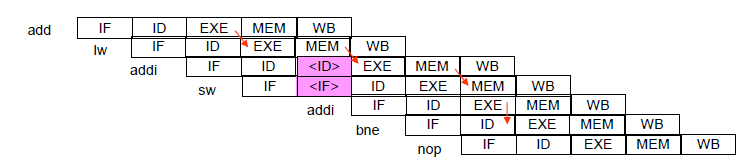
\includegraphics[width=1\textwidth]{im1.png}
    \label{fig:im1}
\end{figure}


Si noti che la dipendenza $1 \rightarrow 4$ non necessita di forwarding, in quanto lo stadio \texttt{WB} dell’istruzione 1 si verifica al 5° ciclo, mentre lo stadio \texttt{ID} dell’istruzione 4 avviene al 6° ciclo. Si noti infine che, poiché per limitare l’hazard sul controllo abbiamo anticipato allo stadio \texttt{ID} del branch il confronto tra i 2 registri (tramite una batteria di porte XOR), per evitare stalli il valore calcolato dall 5° istruzione (\$10) nello stadio \texttt{EXE} deve fluire direttamente nello stadio \texttt{ID} della 6a istruzione. Tale risultato è ottenibile solamente modificando la circuiteria del processore in modo da permettere il recupero del valore calcolato dallo stadio \texttt{EXE} della 5° istruzione nello stadio \texttt{ID} della 6° istruzione. Nel caso non modificassimo la circuiteria andrebbe inserita una \texttt{nop}.

\subsubsection*{Soluzione domanda 2} 
Le uniche dipendenze che non sono risolte dal forwarding (o dal register file speciale) sono quelle tra la \texttt{lw} e l’istruzione successiva ($2 \rightarrow 3$). Un’altra \texttt{nop} bisogna inserirla esplicitamente a causa del delay branch. Abbiamo quindi:
\begin{lstlisting}[numbers=none]
loop:
    add $11, $20, $10
    lw $17, 0($11)
    nop
    addi $17, $17, 50
    sw $17, 0($11)
    addi $10, $10, 4
    bne $10, $21, loop
    nop
\end{lstlisting}
Possiamo ottimizzare il codice, spostando indietro l’istruzione 5 (\texttt{addi}) dopo la \texttt{lw}, in modo da eliminare lo stallo, e l’istruzione 4 (\texttt{sw}) in avanti nel branch delay slot:
\begin{lstlisting}[numbers=none]
loop:
    add $11, $20, $10
    lw $17, 0($11)
    addi $10, $10, 4
    addi $17, $17, 50
    bne $10, $21, loop
    sw $17, 0($11)
\end{lstlisting}


\subsubsection*{Soluzione domanda 3}
Il diagramma relativo al codice non ottimizzato, nel caso in cui il forwarding non fosse attivo, è illustrato (solo parzialmente) di seguito:

\begin{figure}[H]
    \centering
    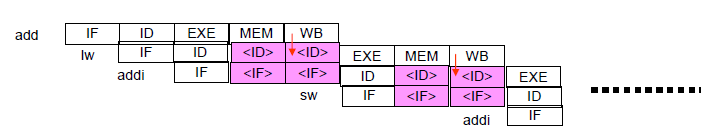
\includegraphics[width=1\textwidth]{im2.png}
   % \caption{Diagramma a più cicli di clock}
    \label{fig:im2}
\end{figure}


Si noti come, grazie al register file speciale (frecce rosse), che scrive un nuovo registro nella prima parte del ciclo, e legge una coppia di registri nella seconda parte dello stesso ciclo, si risparmia un ciclo di stallo.


\newpage

\section*{Risorse}
\begin{itemize}
    \item Struttura e progetto dei calcolatori - David A. Paterson, John L. Hennessy, Capitolo 4. 
\end{itemize}

\subsection*{Risorse WTF}
TIL che qualcuno ha costruito una
\href{https://www.youtube.com/watch?v=LGkkyKZVzug}{ALU-16 bit su Minecraft.} 
\begin{figure}[H]
    \centering
    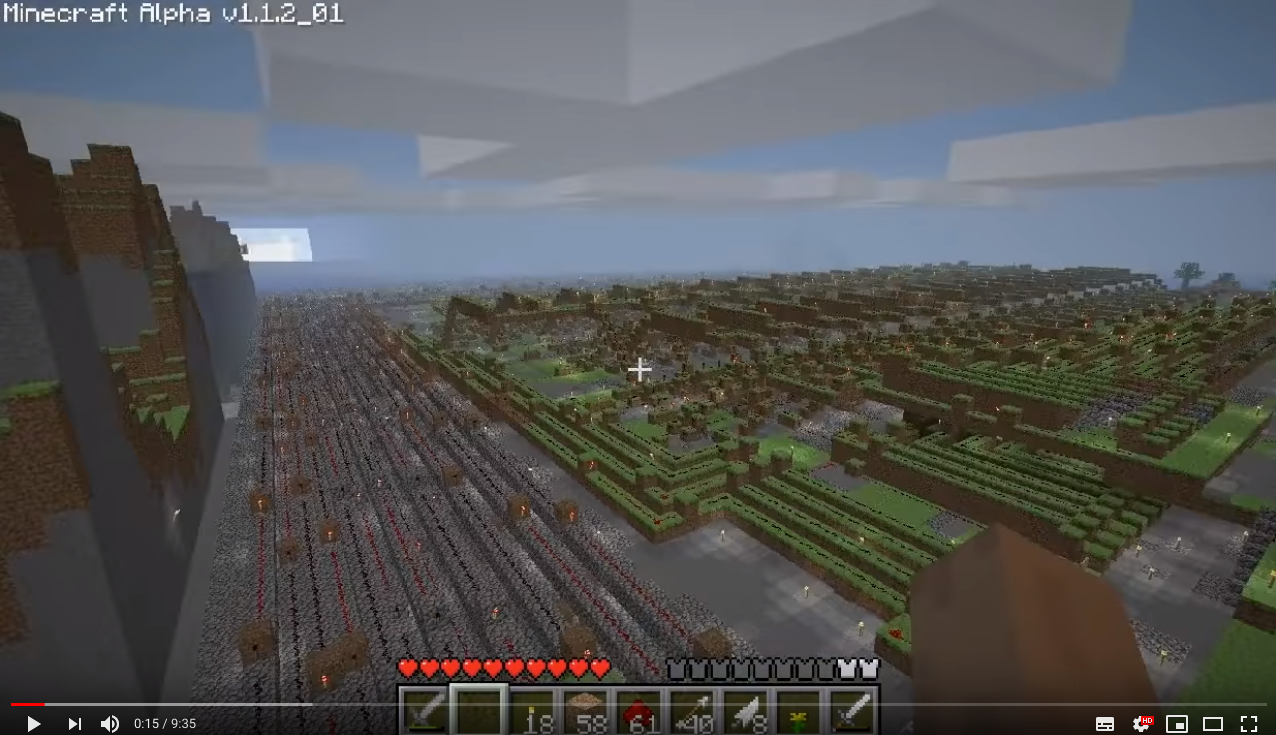
\includegraphics[width=1\textwidth]{im3.png}
\end{figure}
\end{document}
